\documentclass[11pt,compress,t,notes=noshow, aspectratio=169, xcolor=table]{beamer}

\usepackage{../../style/lmu-lecture}
% Defines macros and environments
% This file is included in slides and exercises

% Rarely used fontstyle for R packages, used only in 
% - forests/slides-forests-benchmark.tex
% - exercises/single-exercises/methods_l_1.Rnw
% - slides/cart/attic/slides_extra_trees.Rnw
\newcommand{\pkg}[1]{{\fontseries{b}\selectfont #1}}

% Spacing helpers, used often (mostly in exercises for \dlz)
\newcommand{\lz}{\vspace{0.5cm}} % vertical space (used often in slides)
\newcommand{\dlz}{\vspace{1cm}}  % double vertical space (used often in exercises, never in slides)
\newcommand{\oneliner}[1] % Oneliner for important statements, used e.g. in iml, algods
{\begin{block}{}\begin{center}\begin{Large}#1\end{Large}\end{center}\end{block}}

% Don't know if this is used or needed, remove?
% textcolor that works in mathmode
% https://tex.stackexchange.com/a/261480
% Used e.g. in forests/slides-forests-bagging.tex
% [...] \textcolor{blue}{\tfrac{1}{M}\sum^M_{m} [...]
% \makeatletter
% \renewcommand*{\@textcolor}[3]{%
%   \protect\leavevmode
%   \begingroup
%     \color#1{#2}#3%
%   \endgroup
% }
% \makeatother


\title{Interpretable Machine Learning}
% \author{LMU}
%\institute{\href{https://compstat-lmu.github.io/lecture_iml/}{compstat-lmu.github.io/lecture\_iml}}
\date{}

\begin{document}

\newcommand{\learninggoals}{%
\item Understand fair attribution in cooperative games
\item Learn about Shapley values
}

\lecturechapter{Shapley Values}
\lecture{Interpretable Machine Learning}

% License of titlefigure: free pixabay license
% https://pixabay.com/de/vectors/ergebnis-geld-gesch%C3%A4ft-gehalt-5567652/


\begin{vbframe}{Cooperative Games}
\begin{itemize}
  \item In cooperative games, a set of players of all possible players $P$ with $P = \{1, \hdots, p\}$ forms a coalition $\SsubP$.
  \item A value function $v(S): 2^{|P|}\mapsto \R$ describes the payout (or gain) achieved by any coalition $\forall S \subseteq P$. The value of the empty coalition must be zero: $v(\emptyset) = 0$.
  \item As some players contribute more than others, we are interested to fairly divide the total payout $v(P)$ among the players.
  \item We call the payout per player $\phi_j$, $j \in P$.
  \item What would be properties of a a fair distribution of the payout?
\end{itemize}
\end{vbframe}


\begin{vbframe}{Axioms of Fair Payouts}
  One possibility to define \textbf{fair} payouts are the following axioms for a given value function $v$:
  \begin{itemize}
    \item \textbf{Efficiency}: Player contributions add up to the total payout of the game:
      $\sum\nolimits_{j=1}^p\phi_j = v(P)$
    \item \textbf{Symmetry}: Players $j,k \in P$ who contribute the same to any coalition get the same payout: \\
      If $v(\Scupj) = v(\Scupk)$ for all $\SsubP \setminus\{j,k\}$, then $\phi_j=\phi_k$
    \item \textbf{Dummy / Null Player}: The payout is zero for players who don't contribute to the value of any coalition: \\
      If $v(\Scupj)=v(S)\quad  \forall \quad \SsubP \setminus j$, then $\phi_j=0$
    \item \textbf{Additivity}: For a game $v$ with combined payouts $v(S) = v_1(S) + v_2(S)$, the payout is the sum of payouts: $\phi_{j,v} = \phi_{j,v_1} + \phi_{j, v_2}$
  \end{itemize}

  Is there an attribution formula that adheres to all these axioms?

\end{vbframe}


\begin{vbframe}{Shapley Values}

  Shapley values solve the attribution problem and provide a unique solution given axioms of efficiency, symmetry, dummy and additivity.
\begin{itemize}
  \item Shapley values were proposed by Lloyd Shapley in 1951 for cooperative games (game theory).
  \item The \textbf{Shapley value} assigns a value to each player according to the marginal contribution of each player in all possible coalitions.
  \item $\phi_j = \sum_{\SsubPnoj} \frac{|S|!(|P| - |S| - 1)!}{|P|!}(v(\Scupj) - v(S))$
  \item $v(\Scupj) - v(S)$ is the marginal contribution of player $j$ to coalition $S$.
  \item To compute the Shapley payout for a player, we average, for all possible coalitions, how much the player would increase the value of the coalition (=marginal contribution).
  \item Shapley values are the \textit{only} solution for the attribution with the specified axioms.
\end{itemize}

\tiny{ Shapley, Lloyd S. (August 21, 1951). "Notes on the n-Person Game -- II: The Value of an n-Person Game" (PDF). Santa Monica, Calif.: RAND Corporation.}

\end{vbframe}

\begin{vbframe}{Definition via orders}
The Shapley value was introduced as summation over sets $S$, but it's also possible to define it as a summation of all orders of players.
This also explains where the factor $\frac{|S|!(|P| - |S| - 1)!}{|P|!}$ comes from.
\begin{itemize}
  \item Let $\Pi$ be all possible orders of players ($|P|!$ in total).
  \item Then: $\phi_j = \frac{1}{|P|!} \sum_{\tau \in \Pi} (v(Pre(\tau,j) \cup \{j\}) - v(Pre(\tau,j)))$
  \item $Pre(\tau,j)$ is the set of players before player $j$ in order $\tau$ .
  \item For example players a,b,c: $\Pi = \{(a,b,c), (a,c,b), (b,a,c), (b,c,a), (c,a,b), (c,b,a)\}$. If $\tau = (b,a,c)$ and $j=c$, then $Pre(\tau,j) = \{b, a\}$.
  \item For the Shapley value computation via order definition, we sum the marginal contribution twice for orders that yield set $S = \{a,b\}$, which in the set definition has the weight $2! (3 - 2 - 1)! = 2 \cdot 0! = 2$.
  \item More general, the Shapley value definition via orders is equivalent to the definition via sets, since the number of orders which yield the same coalition $S$ is  $|S|!(|P| - |S| - 1)!$: There are $|S|!$ possible orders of players within coalition $S$ and $(|P| - |S| - 1)!$ possible orders of players without $S$ and $j$.
  \item Relevance of the order definition: The Shapley value can be approximated by sampling permutations. Instead of producing all $|P|!$ permutations, a fixed number of $M$ can be sampled and averaged to approximate the Shapley values.
\end{itemize}

  \begin{tabular}{|c|c|c|c|c|c|c|}
    \multicolumn{3}{c}{\enspace\raisebox{-3.3ex}[0pt][2.6ex]{$ \overbrace{\vphantom{-}\hspace{9em}}^{|S|! \text{ permutations}}$}} &
    \multicolumn{1}{c}{} &
    \multicolumn{3}{c}{\enspace\raisebox{-3.3ex}[0pt][2.6ex]{$ \overbrace{\vphantom{-}\hspace{9em}}^{(|P| - |S| - 1)! \text{ permutations}}$}}\\
    \hline
    $\tau(1)$ & \ldots & $\tau(|S|)$ & $\tau(|S| + 1)$ & $\tau(|S| + 2)$ & \ldots & $\tau(P)$ \\
    \hline
    \multicolumn{3}{c}{\enspace\raisebox{1.3ex}[0pt][2.6ex]{$ \underbrace{\vphantom{-}\hspace{9em}}^{}$}} &
    \multicolumn{1}{c}{\enspace\raisebox{1.3ex}[0pt][2.6ex]{$ \underbrace{\vphantom{-}\hspace{4em}}^{}$}} &
    \multicolumn{3}{c}{\enspace\raisebox{1.3ex}[0pt][2.6ex]{$ \underbrace{\vphantom{-}\hspace{9em}}^{}$}}\\
    \multicolumn{3}{c}{Players before player $j$} & \multicolumn{1}{c}{player $j$} & \multicolumn{3}{c}{Players after player $j$} \\
  \end{tabular}


\end{vbframe}

\frame{
  \frametitle{Shapley Values - Illustration}
The Shapley value of a player $j=2$ is the marginal contribution to the value function when player $2$ enters an abitrary coalition. \\
\only<1>{Here, player $2$ enters the coalition after player $1$, resulting in a value change of $v(\{1,2\}) - v(\{1\}) = 24-12 = 12$. Overall, the coalition has a value of $v(\{1,2,3\}) = 36.$}
\only<2>{We produce all possible orders of player coalitions and measure the value change if player $2$ enters the coalition.}
\begin{center}
  \only<1>{
    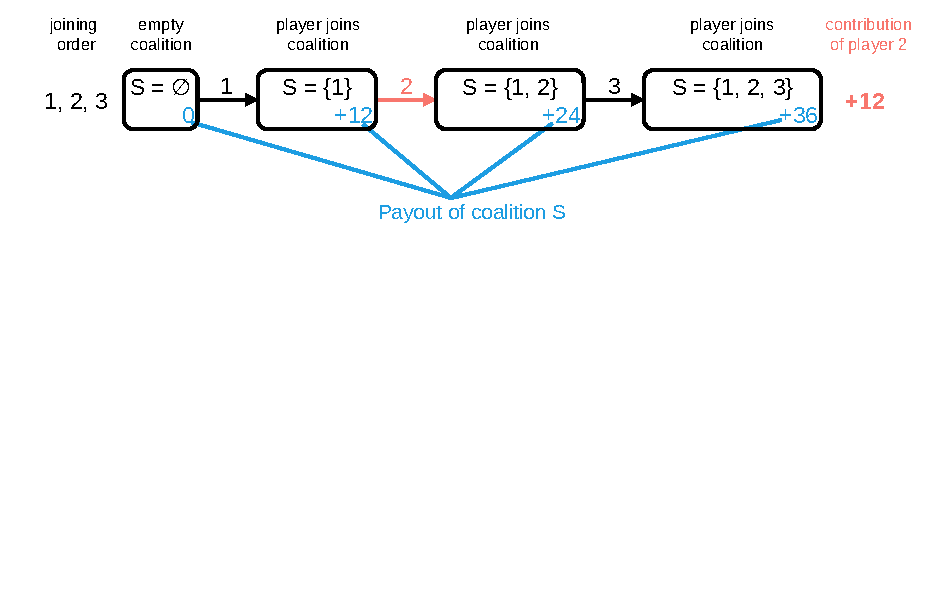
\includegraphics[page=1, width=0.8\textwidth]{figure_man/shapley_feature_effect}
  }
  \only<2>{
    \includegraphics[page=2, width=0.8\textwidth]{figure_man/shapley_feature_effect}
  }
\end{center}

}
\begin{vbframe}{Proof of Axioms}
  The Shapley values fulfills all the 4 axioms.
  Symmetry, Dummy and Additivity are relatively easy to proof:
\begin{itemize}
    % See also: https://math.stackexchange.com/questions/2747088/shapley-value-is-efficient
  \item \textbf{Symmetry}: Let's assume coalition $\SsubPnojk$ and $v(\Scupj) = v(\Scupk)$.
    \begin{itemize}
        \item Then all marginal contributions are equal: $v(\Scupj) -  v(S) = v(\Scupk) -  v(S), \forall \SsubPnojk$
        \item Consequently, $\phi_j = \phi_k$.
    \end{itemize}
  \item \textbf{Dummy}: Let's assume we have player $j$ such that for all $\SsubP$, we have $v(S) = v(\Scupj)$. Then, each marginal contribution of player $j$ is zero, and therefore $\phi_j = 0$.
  \item \textbf{Additivity}:  Assume two games $v_1$ and $v_2$ and a third game which is the sum of both $v(S) = v_1(S) + v_2(S)$. The marginal contribution for all $\SsubPnoj$ for game $v$ can be expressed as $v(\Scupj) - v(S) = v_1(\Scupj) - v_1(S) + v_2(\Scupj) - v_2(S)$. Since the Shapley value is additive in the marginal contributions, we can split the sum into two sums so that $\phi_{j,v} = \phi_{j, v_1} + \phi_{j,v_2}$.
\end{itemize}
Efficiency requires a bit more effort, see proof sketch:
  \begin{itemize}
  \item \textbf{Efficiency}: $v(P)$ exactly appears once per player ($=p$ times) for coalition $S = P \setminus \{j\}$ with the weight $\frac{|P - 1|!(|P| - |P - 1| - 1)!}{|P|!} = \frac{1}{p}$ each. The values for all other coalitions $v(S), \SsubP \{j,k\}$ appear with both minus and plus signs that cancel each other out.
\end{itemize}
\end{vbframe}


\begin{vbframe}{Linearity Axiom Corollary}
  \begin{itemize}
  \item The Shapley values are also linear:
  \item For a game with payout $v(S) = \alpha v_1(S) + v_2(S)$, the Shapley values are $\alpha \phi_{j,v_1} + \phi_{j,v_2}$.
  \item The multiplication with $\alpha$ works since we can pull out $\alpha$ from the sum of marginal contributions, so that for $v(S) = \alpha v_1(S)$ the Shapley value is $\alpha \phi_{j,v_1}$.
  \item We already know that Shapley values are additive which proofs the linearity.
  \end{itemize}
\end{vbframe}



\begin{vbframe}{Applications of Shapley Value}

  \begin{itemize}
      \item Game theory
      \item Economics (e.g., cost allocation)
      \item Marketing (e.g., social network analysis to discover influencers)
      \item ...
      \item Machine learning
       \begin{itemize}
         \item Feature selection: Attribute loss reduction to features.
         \item Quantify data value: Attribute loss reduction to data points.
         \item \textbf{Explain individual predictions}.
       \end{itemize}
  \end{itemize}

  % Economics
  \tiny{Moulin, Hervé. "An application of the Shapley value to fair division with money." Econometrica: Journal of the Econometric Society (1992): 1331-1349.}
% Network analysis
  \tiny{Narayanam, Ramasuri, and Yadati Narahari. "A shapley value-based approach to discover influential nodes in social networks." IEEE Transactions on Automation Science and Engineering 8.1 (2010): 130-147.}
  % Feature Selection
  \tiny{Cohen, Shay B., Eytan Ruppin, and Gideon Dror. "Feature Selection Based on the Shapley Value." IJCAI. Vol. 5. 2005.}
  % Value of data
  \tiny{Ghorbani, Amirata, and James Zou. "Data shapley: Equitable valuation of data for machine learning." International Conference on Machine Learning. PMLR, 2019.}
\end{vbframe}

\endlecture
\end{document}
